\documentclass[11pt,a4paper]{article}
\usepackage[T1]{fontenc}
\usepackage[utf8]{inputenc}
\usepackage{lmodern}
\usepackage[a4paper,margin=2.4cm]{geometry}
\usepackage{microtype}
\usepackage{setspace}
\usepackage{amsmath}
\usepackage{graphicx}
\usepackage{booktabs,tabularx}
\usepackage[table]{xcolor}
\usepackage{caption}
\usepackage{float}
\usepackage{enumitem}
\usepackage{tikz}
\usetikzlibrary{arrows.meta,positioning}
\usepackage{titlesec}
\usepackage{fancyhdr}
\usepackage{lastpage}
\usepackage[hidelinks]{hyperref}

\graphicspath{{../results/figures/}}
\setstretch{1.15}
\setlength{\parindent}{0pt}
\setlength{\parskip}{0.55em}
\captionsetup{font=small,labelfont=bf,labelsep=period}
\setlist{itemsep=0.15em,topsep=0.3em}
\titleformat{\section}{\normalfont\large\bfseries}{\thesection}{0.8em}{}
\titleformat{\subsection}{\normalfont\normalsize\bfseries}{\thesubsection}{0.8em}{}
\titlespacing*{\section}{0pt}{1.3em}{0.5em}
\titlespacing*{\subsection}{0pt}{0.9em}{0.3em}
\definecolor{boxfill}{HTML}{EEF4F6}
\definecolor{edge}{HTML}{1F6F8B}

\pagestyle{fancy}
\fancyhf{}
\fancyhead[L]{\small\itshape Dahal --- Do dermatology VLMs look at the lesion?}
\fancyhead[R]{\small\itshape Preprint, not peer reviewed}
\fancyfoot[C]{\small \thepage\ of \pageref{LastPage}}
\renewcommand{\headrulewidth}{0.4pt}

% set to 1 once the runs are complete and the results section is written
\newif\ifresults
\resultstrue

\begin{document}

\begin{center}
{\LARGE\bfseries Do vision-language models look at the lesion? A counterfactual pilot study of two open models on dermoscopic and smartphone skin images\par}
\vspace{1.0em}
{\large Subarna Dahal\par}
\vspace{0.3em}
{\small Lalitpur, Nepal\quad$\cdot$\quad \href{mailto:dahalsubarna9@gmail.com}{dahalsubarna9@gmail.com}\par}
{\small Code and results: \url{https://github.com/subarna007/derm-vlm-shortcut-pilot}\par}
\vspace{0.3em}
{\small Version of 22 November 2026\par}
\end{center}
\vspace{0.4em}
\noindent\rule{\textwidth}{0.4pt}

{\small
\textbf{Abstract}

\textbf{Background.} Vision-language models (VLMs) now give fluent descriptions and diagnoses for photographs of skin lesions, and medical VLMs are released openly. A fluent answer does not show that it was based on the lesion. Convolutional classifiers for skin cancer are known to use shortcuts such as surgical ink and rulers; whether VLMs do the same has been studied much less, and confident answers that ignore the image would be dangerous in places where a dermatologist is hard to reach.

\textbf{Methods.} Two open models, the medical VLM MedGemma 1.5 4B and the general VLM Qwen2.5-VL 3B, were tested zero-shot on 256 dermoscopic images from Derm7pt and 205 smartphone photos from PAD-UFES-20. Each image was posed as a multiple-choice question with eight diagnoses and the option ``cannot be determined'', and answer probabilities were read from the model's first output token, averaged over two option orders. Four tests were run: (a) the lesion was painted over with surrounding skin; (b) only the skin around the lesion was changed (darker skin tone, surgical-marker ink, or a ruler) while the lesion pixels stayed identical; (c) each model was asked about the seven criteria of the dermoscopic 7-point checklist and its answers were compared with the Derm7pt expert labels; (d) calibration of the token probabilities and of the confidence stated in words was measured with the expected calibration error.

\ifresults
\textbf{Results.} MedGemma was the more accurate model (balanced accuracy 28.0\% on Derm7pt and 43.4\% on PAD-UFES-20, against 20.9\% and 27.7\% for Qwen2.5-VL; chance 12.5\%), and both models called about half of all lesions melanoma. With the lesion painted out, Qwen2.5-VL answered ``cannot be determined'' for 96.7\% of images, but MedGemma still gave a confident diagnosis (top probability at least 50\%) for 50.7\% (95\% CI 45.7--56.1), most often ``nevus'', and its mean confidence fell only from 75.7\% to 70.4\%. Changing only the skin around an unchanged lesion altered MedGemma's diagnosis in 6.2--13.4\% of images and Qwen2.5-VL's in 19.0--29.1\%; a ruler raised MedGemma's probability of melanoma by 1.9 points (1.1--2.8). MedGemma's yes/no answers on the 7-point checklist matched the expert labels better (AUROC 0.52--0.84) than Qwen2.5-VL's (0.46--0.74), and Qwen2.5-VL said ``yes'' to some criteria for almost every image. MedGemma was strongly overconfident (expected calibration error 0.35 and 0.39; mean confidence 68--81\% against accuracy 33--42\%), and so were the confidences both models stated in words.

\textbf{Conclusions.} The medical model is better at reading the lesion but does not know when there is no lesion to read and is far more confident than it is right; the general model is unstable under irrelevant changes. Neither behaviour shows up in an accuracy number. Counterfactual tests like these are cheap and should be reported alongside accuracy for medical VLMs.

\else
\textbf{Results.} The runs are in progress; results will be added when they are complete.
\fi

\textbf{Keywords:} vision-language models; dermatology; shortcut learning; counterfactual evaluation; calibration; MedGemma; Derm7pt; PAD-UFES-20\par
}
\noindent\rule{\textwidth}{0.4pt}

\section{Introduction}

Skin disease is common, and in much of the world a dermatologist is far away. In rural Nepal, for example, a person with a changing mole may have to travel to a city to have it looked at, and many do not. Image-based tools that could help a health worker decide which lesions need referral are therefore attractive, and the last two years have brought a new kind of candidate: vision-language models that take a photograph and answer in text. Some are built for medicine and released openly, such as MedGemma \cite{medgemma2025}; general models such as Qwen2.5-VL \cite{qwen25vl2025} also answer medical questions when asked.

These models write fluently, and that is part of the risk. Earlier work on convolutional classifiers showed that high accuracy in skin cancer detection can rest partly on things that are not the lesion. Purple surgical-marker ink around a lesion made a commercial melanoma classifier more likely to call it melanoma \cite{winkler2019}, rulers in the image changed its output \cite{winkler2021}, and classifiers trained on images with the lesion removed still did far better than chance \cite{bissoto2019}. These are examples of shortcut learning \cite{geirhos2020}: a model uses a feature that is correlated with the label in the training data but is not the reason for the diagnosis. Performance also drops on skin tones that are rare in the training data \cite{daneshjou2022}.

For VLMs there is less evidence. They are trained on very large and mostly unknown image--text collections, so the same shortcuts could have been learned, and their answers come with fluent explanations that can make a wrong answer sound reasonable. Three questions follow from this, and a fourth is about confidence:
\begin{enumerate}[label=\textbf{Q\arabic*.}]
  \item Does a model still give a confident diagnosis when there is no lesion in the image?
  \item Does the diagnosis change when only the skin around the lesion changes?
  \item Do the visual features a model says it sees match what dermatologists annotated?
  \item Does a model's confidence match how often it is right?
\end{enumerate}

This is a pilot: the sample is small, two models are tested, and none is fine-tuned. The aim is to find out whether these problems are present and large enough to justify a full study, and to build a pipeline that can be reused for that study. All code, prompts and per-image answers are public.

\section{Data}

\textbf{Derm7pt} \cite{kawahara2019} contains dermoscopic and clinical images of 1,011 lesions with a diagnosis and expert labels for the seven criteria of the 7-point checklist \cite{argenziano1998}. Its diagnoses were mapped to six of the eight answer options (melanoma, including melanoma metastasis; nevus, including all nevus subtypes; basal cell carcinoma; seborrheic keratosis; dermatofibroma; vascular lesion); lentigo, melanosis and miscellaneous lesions were left out. All basal cell carcinomas, seborrheic keratoses, dermatofibromas and vascular lesions were used, and 60 melanomas and 60 nevi were sampled at random, giving 256 dermoscopic images.

\textbf{PAD-UFES-20} \cite{pacheco2020} contains 2,298 smartphone photographs of 1,641 lesions from a public health programme in Brazil, with six diagnoses: actinic keratosis, basal cell carcinoma, squamous cell carcinoma (including Bowen's disease), seborrheic keratosis, melanoma and nevus. One image per lesion was taken, and 35 lesions per diagnosis were sampled at random (all 30 melanomas that remained after this step were used), giving 205 photographs.

Images were downscaled so that their longest side was at most 896 pixels. Derm7pt is distributed under CC BY-NC-ND 4.0 and PAD-UFES-20 under CC BY 4.0; no Derm7pt images are reproduced in this paper.

\section{Methods}

\subsection{Models and questions}

MedGemma 1.5 4B (\texttt{google/medgemma-1.5-4b-it}) was loaded in 4-bit NF4 quantisation with 32-bit computation, because Gemma~3 models are unstable in 16-bit floating point and the T4 GPUs used do not support bfloat16. Qwen2.5-VL 3B Instruct was loaded in float16 with images resized to at most about 500,000 pixels. Both were run with the Hugging Face \texttt{transformers} library on free Kaggle GPUs, with the same system prompt (``You are an experienced dermatologist.'') and no fine-tuning.

For diagnosis, each image was shown with a multiple-choice question listing the eight diagnoses and a ninth option, ``Cannot be determined from this image'', and the instruction to answer with one letter. Rather than sampling an answer, the probability of each option was read from the logits of the first generated token, restricted to the nine letters. Every question was asked twice, with the eight diagnoses in forward and in reversed order, and the two probability vectors were averaged after mapping letters back to diagnoses; this removes the preference that small models often have for particular letters. The \emph{forced-choice} diagnosis is the most probable of the eight diagnoses, and its probability after renormalising over the eight is the model's \emph{token confidence}. The model \emph{abstains} when ``cannot be determined'' is the most probable of all nine options.

\subsection{Image edits}

Neither dataset has lesion outlines, so a rough mask was made automatically: Otsu thresholding on whichever of two channels (darkness or redness in CIELAB space) separated the image better, keeping the region nearest the centre and filling holes. Masks covering less than 2\% or more than 75\% of the image, or most of its border, were rejected, and all masks were checked by eye on contact sheets. To protect the lesion against an imperfect mask, the mask was enlarged by 12 pixels.

For test (a) the enlarged mask was inpainted from the surrounding skin (Telea's method at reduced resolution, with added skin-like noise). For test (b) three edits changed only pixels outside the enlarged mask: the skin was made darker and browner, faded in over a band to avoid a hard edge; dashed purple surgical-marker lines were drawn around the lesion, as when a lesion is marked for excision; or a ruler with millimetre ticks was drawn along the bottom edge. For every test (b) image the code checks that the pixels inside the enlarged mask are identical to the original.

\subsection{Stated features}

For test (c), each Derm7pt image was shown with seven yes/no questions, one per criterion of the 7-point checklist: atypical pigment network, blue-whitish veil, atypical vascular pattern (dotted or linear irregular vessels), irregular streaks, irregular pigmentation, irregular dots or globules, and regression structures. The probability of ``yes'' was read from the first-token logits and compared with the expert label using the area under the ROC curve. Vascular patterns were grouped as in Kawahara et al.\ \cite{kawahara2019}. Each model also wrote a free-text description of every original image, in a fixed format with the features it used, a diagnosis and a confidence from 0 to 100.

\subsection{Calibration and statistics}

For test (d), the expected calibration error (ECE) was computed with ten equal-width bins \cite{guo2017}, once for the token confidence and once for the confidence the model stated in its free-text answer (using only answers that named a diagnosis). All results are reported with 95\% percentile bootstrap intervals over images (2,000 resamples). Paired comparisons (original against edited image) resample images, keeping both versions of an image together.

\ifresults
\section{Results}
Of the 461 images, 337 had a lesion mask that passed the checks (139 of 256 Derm7pt images and 198 of 205 PAD-UFES-20 images); tests (a) and (b) use these 337, and the other tests use all images. Both models answered every question. The tables below are generated by the analysis code directly from the per-image answers.

\subsection{Diagnosis on the original images}

MedGemma was more accurate than Qwen2.5-VL on both datasets (Table~\ref{tab:baseline}), and both were well above chance but far from useful as a diagnostic tool. Both models over-called melanoma: it was the forced-choice answer for 52\% (MedGemma) and 53\% (Qwen2.5-VL) of the original images, although only 20\% of the sampled lesions were melanomas. Qwen2.5-VL chose ``cannot be determined'' much more often, especially on the smartphone photographs (81.0\%).

\begin{table}[H]\centering\small
\caption{Diagnosis on the original images, forced choice among 8 diagnoses (\%, 95\% bootstrap interval). Chance balanced accuracy is 12.5\%.}\label{tab:baseline}
\begin{tabular}{lcc}\toprule
 & MedGemma 1.5 4B & Qwen2.5-VL 3B \\\midrule
\textit{derm7pt} ($n=256$) &  &  \\
\quad Accuracy & 33.2 (27.3--39.1) & 27.7 (21.9--33.2) \\
\quad Balanced accuracy & 28.0 (23.8--32.0) & 20.9 (18.2--23.9) \\
\quad Answered ``cannot be determined'' & 9.0 & 30.5 \\
\textit{pad} ($n=205$) &  &  \\
\quad Accuracy & 42.4 (36.1--49.3) & 27.8 (21.5--34.1) \\
\quad Balanced accuracy & 43.4 (38.7--48.4) & 27.7 (21.9--33.5) \\
\quad Answered ``cannot be determined'' & 29.8 & 81.0 \\
\bottomrule\end{tabular}\end{table}

\begin{table}[H]\centering\small
\caption{Test (a): the lesion is painted over with surrounding skin (\%). A confident diagnosis means not answering ``cannot be determined'' and giving the top diagnosis at least 50\% probability.}\label{tab:removed}
\begin{tabular}{lcc}\toprule
 & MedGemma 1.5 4B & Qwen2.5-VL 3B \\\midrule
Images & 337 & 337 \\
``Cannot be determined'', original & 18.4 (14.2--22.6) & 59.9 (54.6--65.0) \\
``Cannot be determined'', lesion removed & 48.1 (42.7--53.1) & 96.7 (94.7--98.5) \\
Confident diagnosis with lesion removed & 50.7 (45.7--56.1) & 2.4 (0.9--4.2) \\
Same diagnosis as on the original & 32.6 (27.6--37.7) & 30.3 (25.5--35.6) \\
Accuracy, original $\rightarrow$ lesion removed & 39.5 $\rightarrow$ 28.8 & 29.1 $\rightarrow$ 15.7 \\
\bottomrule\end{tabular}\end{table}

\begin{table}[H]\centering\small
\caption{Test (b): only the skin around the lesion is changed; lesion pixels are identical (\%, 95\% bootstrap interval).}\label{tab:background}
\begin{tabular}{lcc}\toprule
 & MedGemma 1.5 4B & Qwen2.5-VL 3B \\\midrule
\textit{Darker skin} &  &  \\
\quad Diagnosis changed & 13.4 (9.8--17.2) & 29.1 (24.3--34.1) \\
\quad Change in P(melanoma), points & +0.7 (-0.7 to +2.1) & +2.3 (+1.2 to +3.4) \\
\textit{Skin marker} &  &  \\
\quad Diagnosis changed & 10.1 (7.1--13.4) & 23.7 (19.3--28.2) \\
\quad Change in P(melanoma), points & -0.1 (-1.0 to +0.8) & +0.7 (-0.2 to +1.5) \\
\textit{Ruler} &  &  \\
\quad Diagnosis changed & 6.2 (3.9--8.9) & 19.0 (14.8--23.1) \\
\quad Change in P(melanoma), points & +1.9 (+1.1 to +2.8) & +1.1 (+0.4 to +1.8) \\
\bottomrule\end{tabular}\end{table}

\begin{table}[H]\centering\small
\caption{Test (c): AUROC of the model's yes-probability for each 7-point checklist criterion against the Derm7pt expert label (95\% bootstrap interval; 0.5 is chance). Prevalence in brackets.}\label{tab:criteria}
\begin{tabular}{lcc}\toprule
 & MedGemma 1.5 4B & Qwen2.5-VL 3B \\\midrule
atypical network (17\%) & 0.81 (0.74--0.86) & 0.67 (0.58--0.75) \\
blue white veil (20\%) & 0.84 (0.79--0.89) & 0.74 (0.66--0.82) \\
atypical vascular (5\%) & 0.62 (0.45--0.76) & 0.66 (0.52--0.80) \\
irregular streaks (20\%) & 0.75 (0.69--0.82) & 0.59 (0.50--0.67) \\
irregular pigmentation (33\%) & 0.77 (0.71--0.83) & 0.59 (0.51--0.66) \\
irregular dots (46\%) & 0.62 (0.56--0.69) & 0.55 (0.48--0.63) \\
regression (20\%) & 0.52 (0.44--0.61) & 0.46 (0.37--0.54) \\
\bottomrule\end{tabular}\end{table}

\begin{table}[H]\centering\small
\caption{Test (d): calibration on the original images (expected calibration error, 10 bins).}\label{tab:calibration}
\begin{tabular}{lcc}\toprule
 & MedGemma 1.5 4B & Qwen2.5-VL 3B \\\midrule
\textit{derm7pt} &  &  \\
\quad Accuracy / mean token confidence & 33.2 / 68.3 & 27.7 / 51.1 \\
\quad Token ECE & 0.35 (0.29--0.41) & 0.23 (0.18--0.29) \\
\quad Verbal ECE (answers naming a diagnosis) & 0.61 (0.55--0.67) (242/256) & 0.53 (0.36--0.68) (36/256) \\
\textit{pad} &  &  \\
\quad Accuracy / mean token confidence & 42.4 / 80.6 & 27.8 / 32.7 \\
\quad Token ECE & 0.39 (0.32--0.45) & 0.08 (0.05--0.14) \\
\quad Verbal ECE (answers naming a diagnosis) & 0.45 (0.37--0.52) (156/205) & 0.67 (0.46--0.84) (19/205) \\
\bottomrule\end{tabular}\end{table}


\subsection{(a) Lesion removed}

The two models behaved very differently when the lesion was painted out (Table~\ref{tab:removed}, Figure~\ref{fig:removed}). Qwen2.5-VL answered ``cannot be determined'' for 96.7\% of these images and gave a confident diagnosis for only 2.4\%. MedGemma abstained for 48.1\% and gave a confident diagnosis for 50.7\%; its mean confidence in its top diagnosis fell only from 75.7\% to 70.4\%. With the lesion removed, MedGemma's answer was usually ``nevus'' (71\% of Derm7pt images and 52\% of PAD-UFES-20 images, where ``basal cell carcinoma'' made up most of the rest). Its accuracy on Derm7pt images without a lesion (35.3\%) was close to what always answering ``nevus'' would give in that subset (30.2\%), so the remaining accuracy reflects a default answer rather than information in the surrounding skin.

\begin{figure}[H]\centering
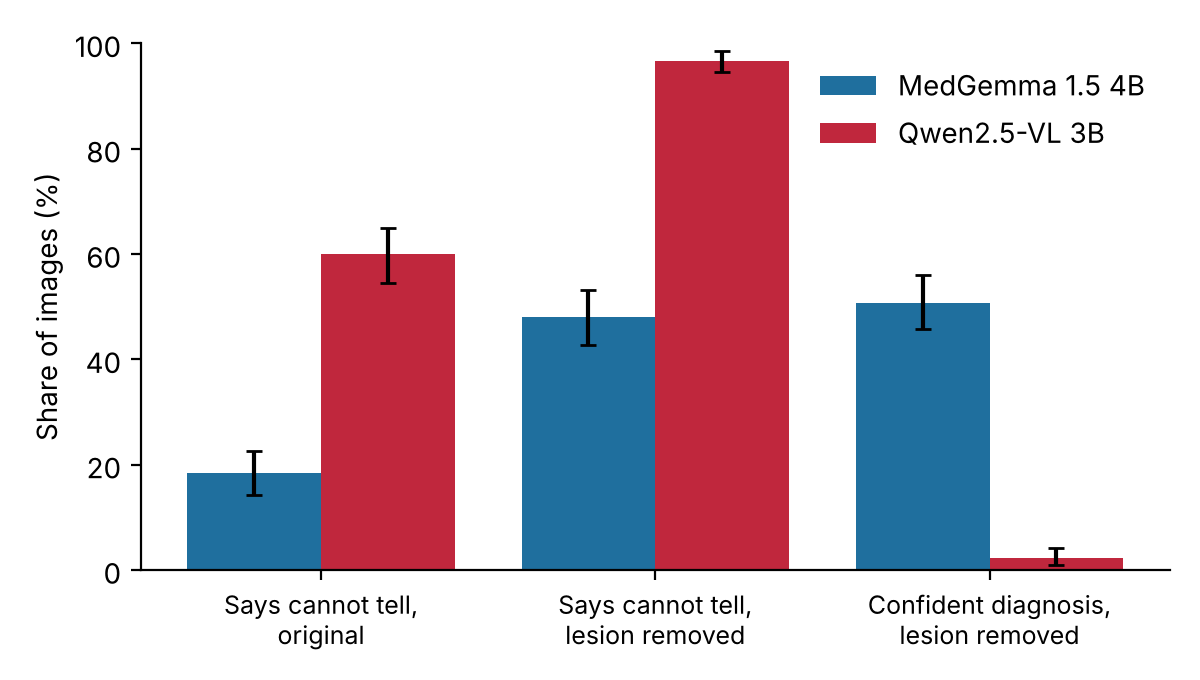
\includegraphics[width=0.72\textwidth]{lesion_removed.png}
\caption{Test (a). Share of images on which each model answers ``cannot be determined'', before and after the lesion is painted out, and share on which it still gives a confident diagnosis (top probability at least 50\%). 95\% bootstrap intervals; $n=337$.}\label{fig:removed}
\end{figure}

\subsection{(b) Background changed, lesion unchanged}

Every background edit changed some diagnoses even though the lesion pixels were identical (Table~\ref{tab:background}, Figure~\ref{fig:background}). Qwen2.5-VL was the less stable model: 29.1\% of its diagnoses changed when the surrounding skin was darkened, 23.7\% with skin-marker lines and 19.0\% with a ruler. For MedGemma the figures were 13.4\%, 10.1\% and 6.2\%. The edits moved the probability of melanoma only slightly on average. The clearest effects were a ruler raising MedGemma's probability of melanoma by 1.9 points (95\% CI 1.1--2.8) and darker skin raising Qwen2.5-VL's by 2.3 points (1.2--3.4); skin-marker lines did not move either model's melanoma probability measurably. Accuracy changed little, which means the changed diagnoses were mostly swaps between wrong answers or between a right and a wrong one in both directions.

\begin{figure}[H]\centering
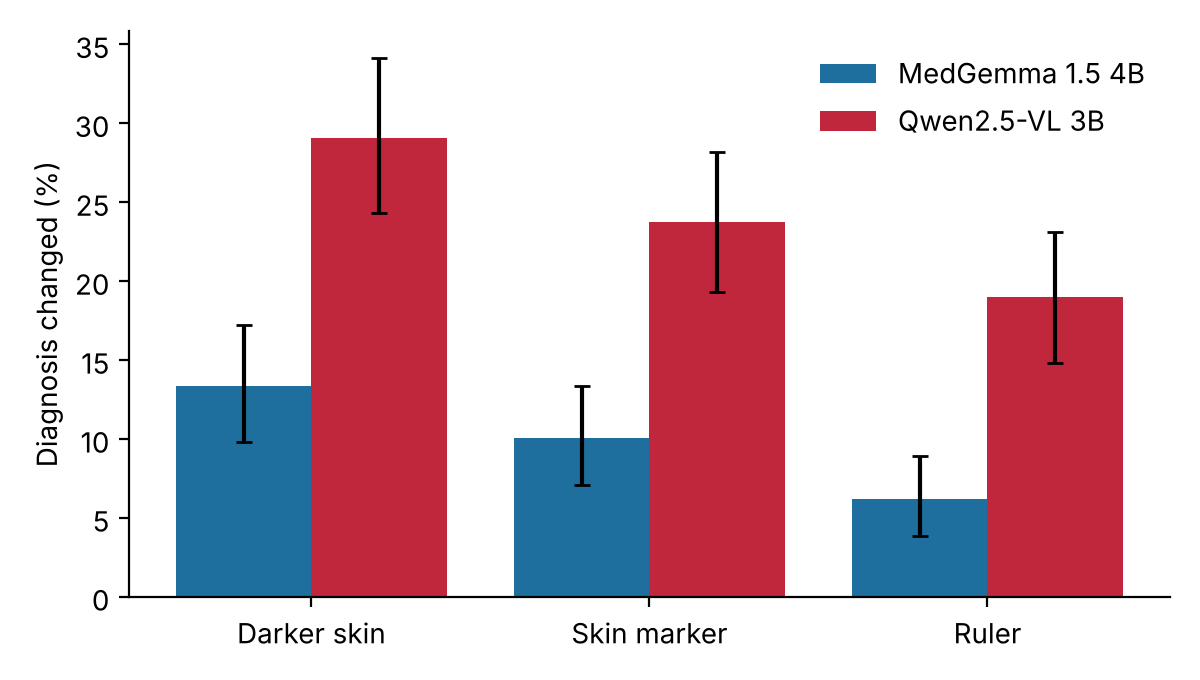
\includegraphics[width=0.66\textwidth]{background_flips.png}
\caption{Test (b). Share of images whose forced-choice diagnosis changed after an edit that left the lesion pixels untouched. 95\% bootstrap intervals; $n=337$ per edit.}\label{fig:background}
\end{figure}

\subsection{(c) Stated features}

MedGemma's answers on the seven checklist criteria matched the expert labels better than Qwen2.5-VL's for six of the seven criteria (Table~\ref{tab:criteria}, Figure~\ref{fig:criteria}); its best were blue-whitish veil (AUROC 0.84) and atypical pigment network (0.81). Regression structures were not recognised by either model (0.52 and 0.46). Both models said ``yes'' far more often than the criteria occur: Qwen2.5-VL said yes to irregular dots or globules for every image and to irregular pigmentation and atypical network for 99\%, while their prevalence was 47\%, 33\% and 17\%. A model's own checklist was linked to its own diagnosis much more strongly for MedGemma (Spearman correlation between the summed criterion probabilities and its melanoma probability 0.71) than for Qwen2.5-VL (0.25).

\begin{figure}[H]\centering
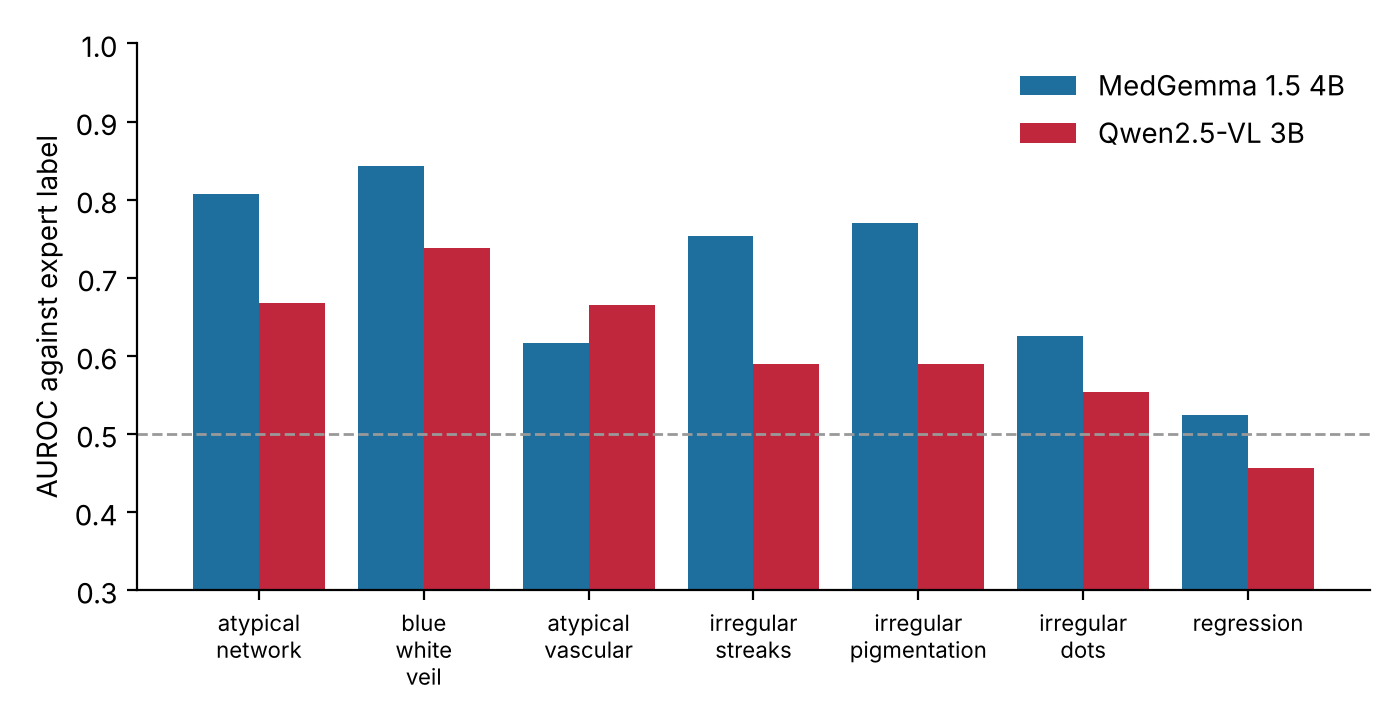
\includegraphics[width=0.72\textwidth]{criteria_auroc.png}
\caption{Test (c). AUROC of each model's yes-probability against the Derm7pt expert label for the seven criteria of the 7-point checklist ($n=256$). The dashed line is chance.}\label{fig:criteria}
\end{figure}

\subsection{(d) Calibration}

MedGemma was strongly overconfident (Table~\ref{tab:calibration}, Figure~\ref{fig:reliability}): its mean token confidence was 68.3\% on Derm7pt and 80.6\% on PAD-UFES-20, against accuracies of 33.2\% and 42.4\% (ECE 0.35 and 0.39). Qwen2.5-VL was overconfident on Derm7pt (51.1\% against 27.7\%, ECE 0.23) but close to calibrated on PAD-UFES-20 (ECE 0.08), where it was rarely confident at all. Confidence stated in words was worse for both models. MedGemma named a diagnosis in its free-text answer for 242 of 256 Derm7pt and 156 of 205 PAD-UFES-20 images, with ECE 0.61 and 0.45; Qwen2.5-VL named one for only 36 and 19 images, so its verbal calibration rests on very few answers.

\begin{figure}[H]\centering
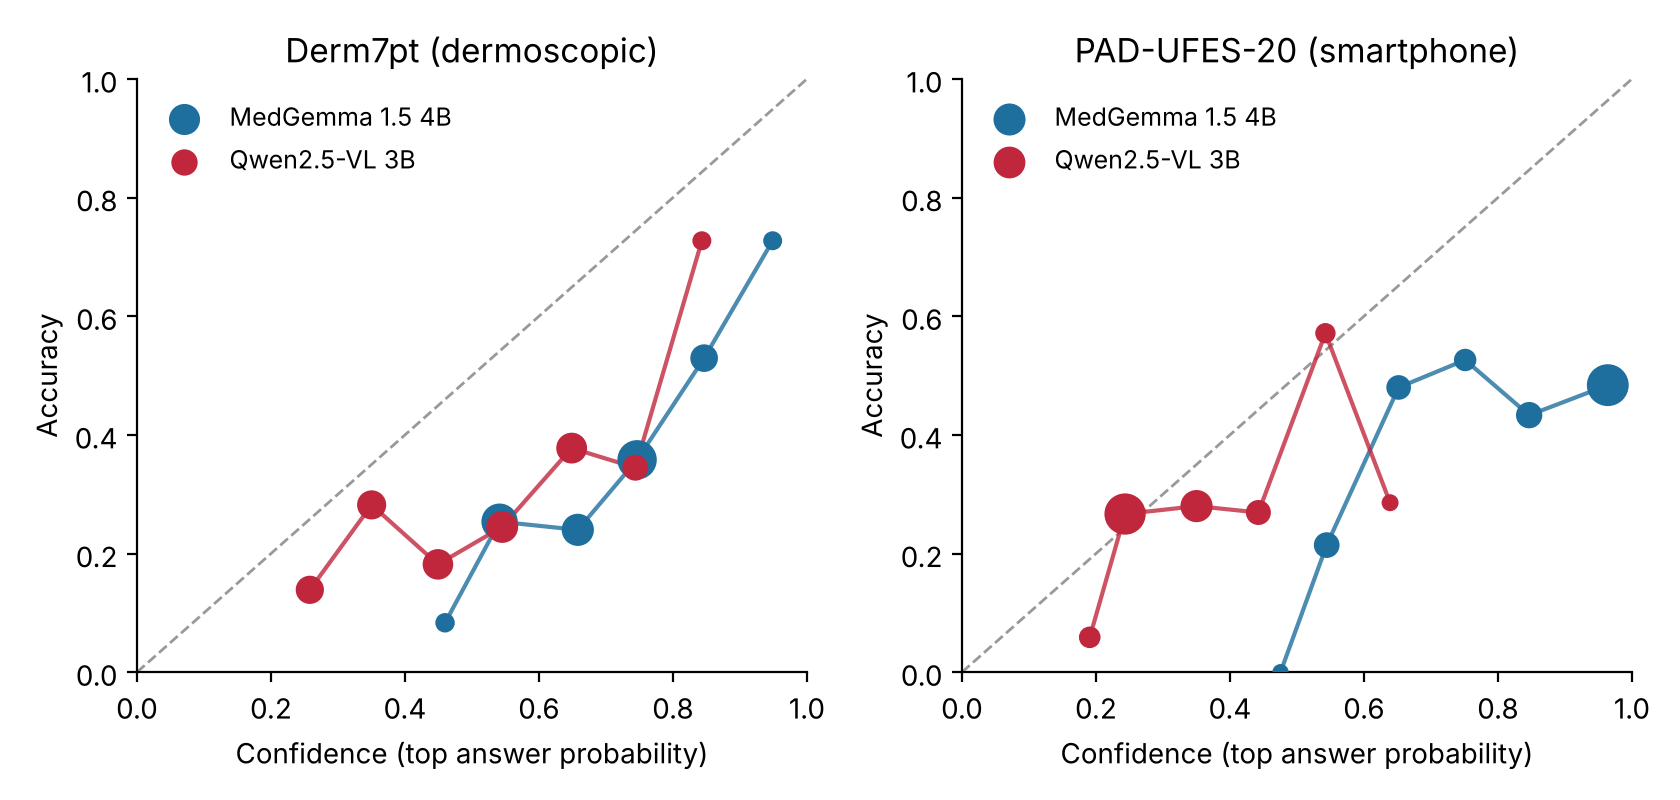
\includegraphics[width=0.9\textwidth]{reliability.png}
\caption{Test (d). Reliability diagrams for the token confidence on the original images; marker size shows the number of images in a bin, and bins with fewer than five images are not drawn. A calibrated model lies on the dashed line.}\label{fig:reliability}
\end{figure}


\section{Discussion}
The two models fail in opposite ways. MedGemma, trained on medical images, is clearly better at reading the lesion: it is more accurate, more stable when the background changes, and its answers about dermoscopic structures agree better with dermatologists. But it does not recognise when there is nothing to read. With the lesion gone it still gives a confident answer for half the images, and across all images it is roughly twice as confident as it is right. Qwen2.5-VL is the opposite: it is cautious, often to the point of declining to answer, and it almost always notices that the lesion is missing, but its diagnoses change for a quarter of images when only the surrounding skin is edited, and its feature answers are close to ``yes to everything''.

None of this is visible in an accuracy number. A user who saw only that MedGemma reaches 43\% balanced accuracy on smartphone photos would not learn that, on photos with the lesion painted out, its average confidence in its top diagnosis is still 70\%. For the use that motivates this work, a referral aid for health workers far from a dermatologist, that is the failure that matters most: a confident wrong answer is worse than ``I cannot tell''. The lesion-removal and background tests cost a few lines of image processing and one extra model call per image, and they could be reported alongside accuracy for any medical VLM.

Some results are smaller than expected. Earlier work found that surgical-marker ink pushed a convolutional classifier towards melanoma \cite{winkler2019}; here marker lines changed diagnoses but did not move the melanoma probability of either model measurably, while a ruler did for MedGemma. The skin-tone edit is crude, so the effect of darker skin on Qwen2.5-VL should be checked with real images of darker skin before drawing any conclusion about fairness.

The pilot suggests three directions for a full study: (1) training or prompting methods that let a model abstain when the lesion is missing or unclear, evaluated with exactly these counterfactual tests; (2) grounding the model's stated features in the image, for example by asking it to point to each structure and checking the location against a segmentation; and (3) repeating the tests on larger and fine-tuned models and on images from South Asian patients, where none of the public datasets used here applies.

\fi

\section{Limitations}

The sample is small, so the intervals are wide; the study can show whether an effect is large, not rank models precisely. Only two small open models were tested, zero-shot and with one prompt, so the results do not describe larger or fine-tuned models. The lesion masks come from thresholding, not from experts, and the 12-pixel margin means that the darker-skin edit leaves a band of original skin around the lesion. Inpainting removes the lesion but leaves a smooth patch that is not quite like skin, so some ``cannot be determined'' answers in test (a) may be a reaction to the patch rather than to the missing lesion. The skin-tone edit changes colour only, which is a crude stand-in for darker skin. Reading answers from the first token assumes the model would answer with a letter; a model that would have started with ``The answer is'' is still scored on the letter it gives most probability to. Finally, Derm7pt and PAD-UFES-20 come from Europe and Brazil; neither represents patients in Nepal.

\section*{Code and data availability}

Code, prompts, per-image model answers and the analysis are at\\\url{https://github.com/subarna007/derm-vlm-shortcut-pilot}. Derm7pt is available after registration from Simon Fraser University and PAD-UFES-20 from Mendeley Data.

\begin{thebibliography}{99}\small
\bibitem{medgemma2025} Sellergren A, et al. MedGemma technical report. arXiv:2507.05201; 2025.
\bibitem{qwen25vl2025} Bai S, Chen K, Liu X, et al. Qwen2.5-VL technical report. arXiv:2502.13923; 2025.
\bibitem{winkler2019} Winkler JK, Fink C, Toberer F, et al. Association between surgical skin markings in dermoscopic images and diagnostic performance of a deep learning convolutional neural network for melanoma recognition. JAMA Dermatology. 2019;155(10):1135--1141.
\bibitem{winkler2021} Winkler JK, Sies K, Fink C, et al. Association between different scale bars in dermoscopic images and diagnostic performance of a market-approved deep learning convolutional neural network for melanoma recognition. European Journal of Cancer. 2021;145:146--154.
\bibitem{bissoto2019} Bissoto A, Fornaciali M, Valle E, Avila S. (De)constructing bias on skin lesion datasets. In: Proceedings of the IEEE/CVF Conference on Computer Vision and Pattern Recognition Workshops; 2019.
\bibitem{geirhos2020} Geirhos R, Jacobsen JH, Michaelis C, Zemel R, Brendel W, Bethge M, Wichmann FA. Shortcut learning in deep neural networks. Nature Machine Intelligence. 2020;2:665--673.
\bibitem{daneshjou2022} Daneshjou R, Vodrahalli K, Novoa RA, et al. Disparities in dermatology AI performance on a diverse, curated clinical image set. Science Advances. 2022;8(31):eabq6147.
\bibitem{kawahara2019} Kawahara J, Daneshvar S, Argenziano G, Hamarneh G. Seven-point checklist and skin lesion classification using multitask multimodal neural nets. IEEE Journal of Biomedical and Health Informatics. 2019;23(2):538--546.
\bibitem{argenziano1998} Argenziano G, Fabbrocini G, Carli P, et al. Epiluminescence microscopy for the diagnosis of doubtful melanocytic skin lesions: comparison of the ABCD rule of dermatoscopy and a new 7-point checklist based on pattern analysis. Archives of Dermatology. 1998;134(12):1563--1570.
\bibitem{pacheco2020} Pacheco AGC, Lima GR, Salom\~ao AS, Krohling B, et al. PAD-UFES-20: a skin lesion dataset composed of patient data and clinical images collected from smartphones. Data in Brief. 2020;32:106221.
\bibitem{guo2017} Guo C, Pleiss G, Sun Y, Weinberger KQ. On calibration of modern neural networks. In: Proceedings of the 34th International Conference on Machine Learning. PMLR 70; 2017. p. 1321--1330.
\end{thebibliography}

\end{document}
